\title{Question 5}
\author{Anshika Raman \\ Roll No: 210050014
    \and Kushal Aggarwal \\ Roll No: 210100087
    \and Kavan Vavadiya \\ Roll No: 210100166}


\documentclass[11pt]{article}
\usepackage{graphicx, caption}
\usepackage{amsmath}
\usepackage{amssymb}
\usepackage{hyperref}
\usepackage{ulem}
\usepackage[margin=0.5in]{geometry}
\begin{document}
\maketitle

\begin{enumerate}
\item[Que 5.]
\begin{enumerate}

\item[(c)] \
\begin{figure}[!htb]
\centering
\minipage{0.5\textwidth}
  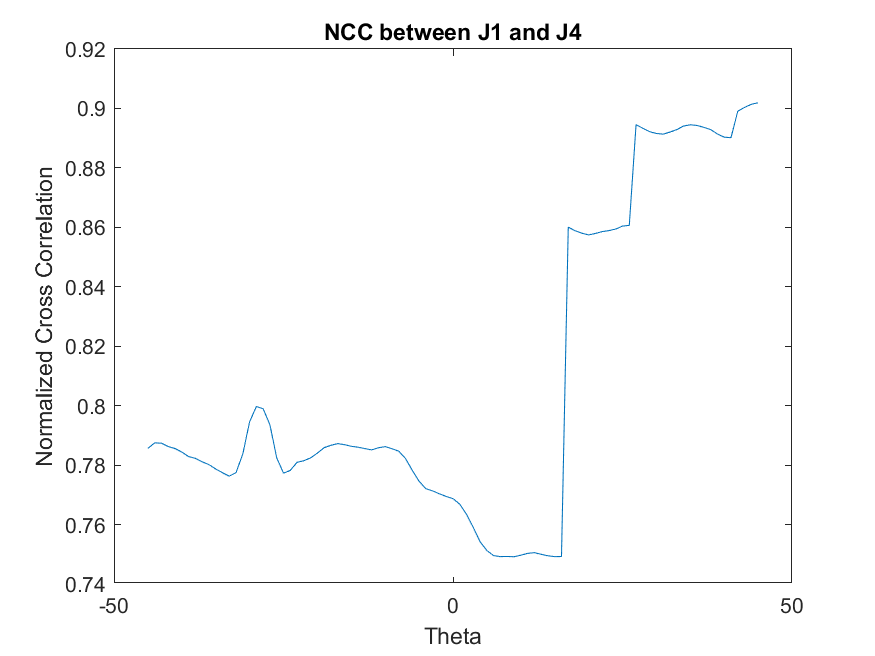
\includegraphics[width=100mm]{images/NCC.png}
  \caption*{Normalized Cross Correlation}
  \endminipage\hfill
  \minipage{0.5\textwidth}
 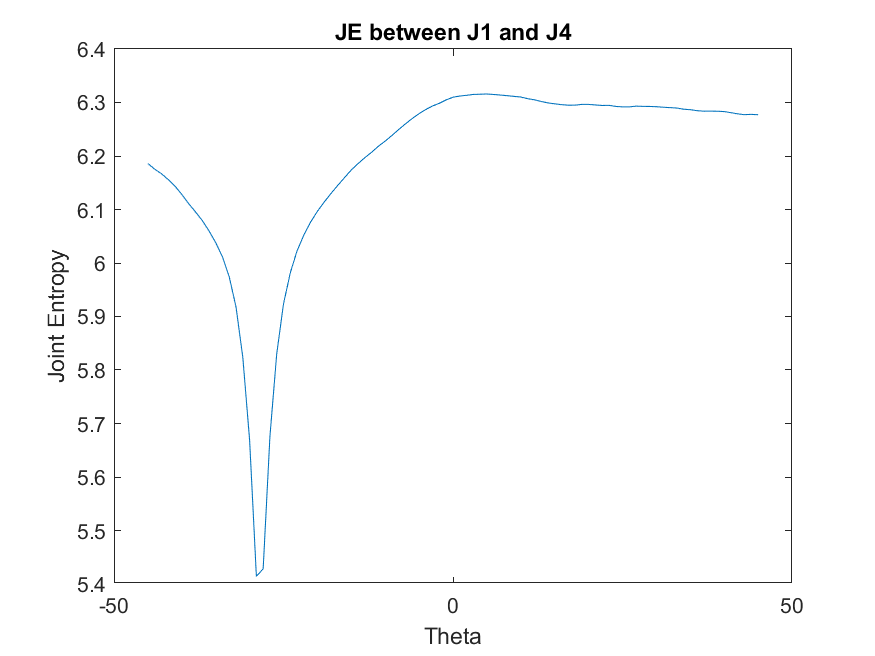
\includegraphics[width=100mm]{images/JE.png}
  \caption*{Joint Entropy}
    \endminipage\hfill
  \minipage{0.5\textwidth}
  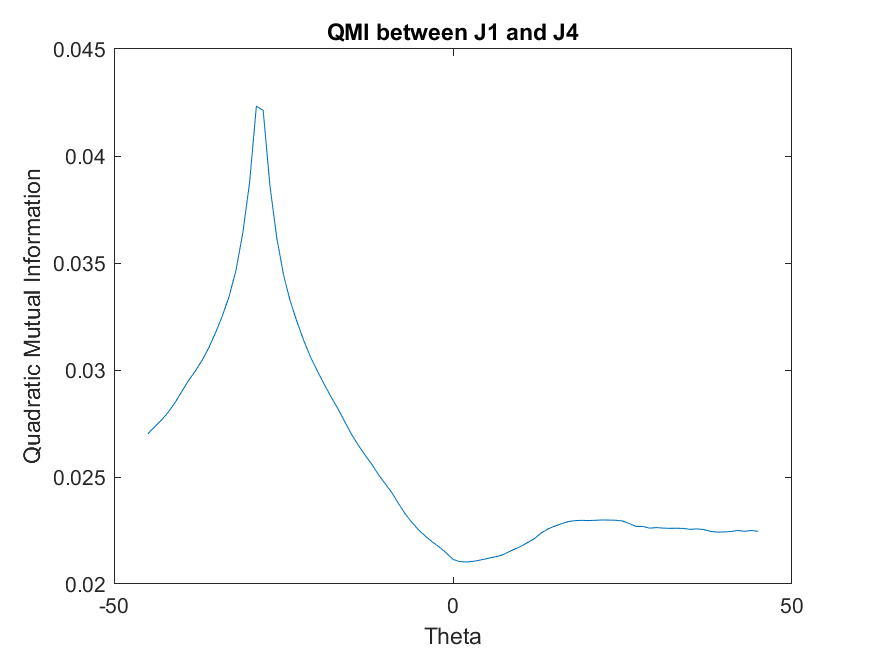
\includegraphics[width=100mm]{images/QMI.png}
  \caption*{Quadratic Mutual Information}
  \endminipage\hfill
\caption{Nearest neighbour interpolation}
\end{figure}

\pagebreak
\item [(d)] \
\begin{itemize}
  \item We select the angle $\theta$ that maximizes the \textbf{NCC (Normalized Cross-Correlation)}. According to the plot, NCC peaks at $\theta = 45.0^\circ$, but this is evidently not the correct rotation angle. Although there is a local maximum at $-29^\circ$, it is not the global maximum. This suggests that NCC may not be a reliable measure for all types of image alignment.
  \item We choose the angle $\theta$ that minimizes \textbf{JE (joint energy)}. The plot indicates that the minimum of JE occurs at $\theta = -29^\circ$, which is close to the expected value. Given that the initial rotation was 28.5° (with counterclockwise as positive) and the step size for $\theta$ is 1°, we have determined the answer with a precision of up to 1 degree.
  \item  We select the angle $\theta$ that maximizes \textbf{QMI (Quadratic Mutual Information)}. According to the plot, the maximum of QMI occurs at $\theta = -29^\circ$, which is near the expected value. Given that the initial rotation was 28.5° (with counterclockwise as positive) and the step size for $\theta$ is 1°, we achieved a precision of up to 1 degree in our result
\end{itemize}

\item [(e)] \
The optimal rotation according to JE, is $-29^\circ$.
\begin{figure}[!htb]
\centering
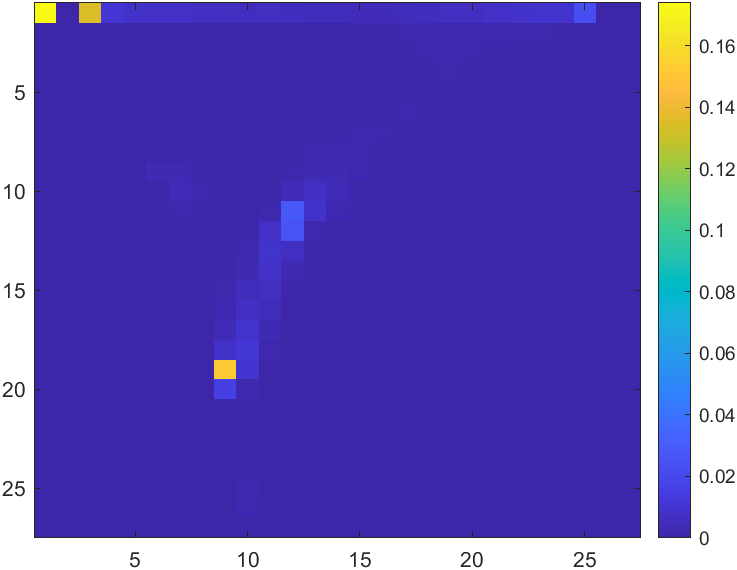
\includegraphics[width=100mm]{images/op_JE_hist.png}
\end{figure}
\item [(f)] \
When two random variables, \( I_1 \) and \( I_2 \), are independent, their joint probability distribution \( P_{I_1, I_2}(i_1, i_2) \) equals the product of their marginal distributions \( P_{I_1}(i_1) \) and \( P_{I_2}(i_2) \):

\[
P_{I_1, I_2}(i_1, i_2) = P_{I_1}(i_1) P_{I_2}(i_2).
\]

Thus, the greater the magnitude of the difference between \( P_{I_1, I_2}(i_1, i_2) \) and \( P_{I_1}(i_1) P_{I_2}(i_2) \), the stronger the dependence between the variables. Consequently, the images are more dependent (or correlated) when the QMI, given by

\[
\text{QMI} = \sum_{i_1} \sum_{i_2} \left( P_{I_1, I_2}(i_1, i_2) - P_{I_1}(i_1) P_{I_2}(i_2) \right)^2,
\]

is larger. Therefore, image alignment is achieved when their QMI is maximized.

\end{enumerate}
\end{enumerate}

\end{document}